\subsection{Introduction}

SWOT stands for Strengths, Weaknesses, Opportunities, and Threats, SWOT Analysis helps you define
what your business is better at and what it is lacking from.

By analysing and studying your business you will run into some questions like:
{
\renewcommand\labelitemi{}
\begin{itemize}
    \item what do you have?
    \item what do you miss?
    \item what is open for you?
    \item what may harm your business in the future?
\end{itemize}
}
all these questions can be answered by providing a suitable SWOT Analysis of your business.

\begin{figure}[h]
    \centering
    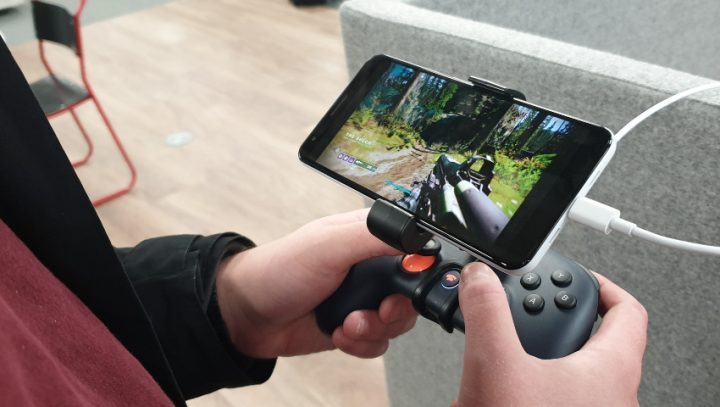
\includegraphics[width=0.8\textwidth]{images/stream.jpg}
    \caption{Stadia Game Stream}
    \label{fig:stream}
\end{figure}

\subsection{Strengths}
    \begin{itemize}
        \item \textbf{Gaming Experience:}
            Google Stadia offers a very well-established gaming stream for 
            their users, no delay or frame-drop, and the game controller is immediately reflected.
        \item \textbf{Google Image:}
            Google itself is the most clicked (visited) search-engine in the world
            this gives Stadia a great advantage since it's related to Google; on the contrary, companies
            like \emph{Tencent} and \emph{Walmart} will struggle more in marketing their competing product (service).
        \item \textbf{Content Creators:} 
            nowadays we have a large number of YouTubers (content creators), who stream their games and 
            upload it on their channels, since YouTube is one of Google's corporations Google Stadia
            easily offers full integration with YouTube for content, so no license are required, and 
            it becomes easily to upload your content.
    \end{itemize}

\subsection{Weaknesses}
\begin{itemize}    
    \item \textbf{Fiber:} 
        most of the world has turned their cables from TCP to Fiber however, some countries are still using
        old cable technologies, unfortunately Google Stadia requires the usage of Fiber cables,
        not only fast internet connection with $20mbs$, but also having Fiber cables.
    \item \textbf{Online Gaming:}
        even though Stadia offers a very good experience when playing, but sometimes the game controller
        may not be reflected, and the game may not respond, in offline games this is not a big issue, as you
        can respawn to your last checkpoint, but in online gaming this issue may but Stadia out of business.
    \item \textbf{Pricing:}
        as explained before, Stadia requires monthly fee and games are purchased separately, this demerit affect 
        gamers mostly, many people are purchasing gaming consoles (PS, XBOX) or even upgrading their PC for better gaming
        experience, and then purchase video games separately, so without a price plan for video games, Stadia is not
        offering them so much.
\end{itemize}

\subsection{Opportunities}
\begin{itemize}    
    \item \textbf{Unique:} 
        Google Stadia's strengths majorly lies in the uniqueness of their service,
        Cloud Gaming business is a brand new service not so many companies are competing in this
        area yet.

    \item \textbf{Leadership:}
        Stadia is the first of its kind, no major competitors yet, so they can add more features and obtain license for them
        before any other company does.
    
    \item \textbf{Gaming:}
        in total, there were an estimated 2.7 billion gamers across the globe in 2020, this creates a major opportunity
        for companies like Stadia.

    \item \textbf{Evolution:}
        as time goes by video games are evolving, and to have the best gaming experience you need to purchase the
        most recent gaming console, these consoles cost a lot, Stadia here appears to be a better solution
        for providing the same (sometimes better) gaming experience without the need of purchasing newer gaming
        consoles, so in order to achieve that they need to be always updated with the best technology.
\end{itemize}

\subsection{Threats}
\begin{itemize}    
    \item \textbf{Competitors:}
        the arising of other companies like Amazon and Microsoft, these major companies will have to compete against
        Stadia one day, and as huge as they are they will also come up with a huge marketing plan, and even better 
        promotion and pricing plans to overcome Stadia.

    \item \textbf{Gaming Consoles:}
        PS, XBOX and other companies can have similar   approach as google Stadia, allowing the user to play online 
        without the need of purchasing new gaming consoles, and overcome the problems google Stadia has regarding 
        online gaming.
\end{itemize}